\chapter{Ausarbeitung}
\section{Aufgabe 1}
In dieser Aufgabe wird eine pr"azise Positionsberechnung auf der Referenzstation durchgef"uhrt. Wenn man alle Satelliten genommen hat, ist das Ergebnis der Bewegung falsch. Der Grund daf"ur sind die Beidou Satelliten, die werden bei der Auswertung vernachl"assigt. \autoref{fig:bewegung}
\begin{figure}[ht]\centering 
	\subfigure[mit Beidou (Gitter L"anger 1cm)]{
		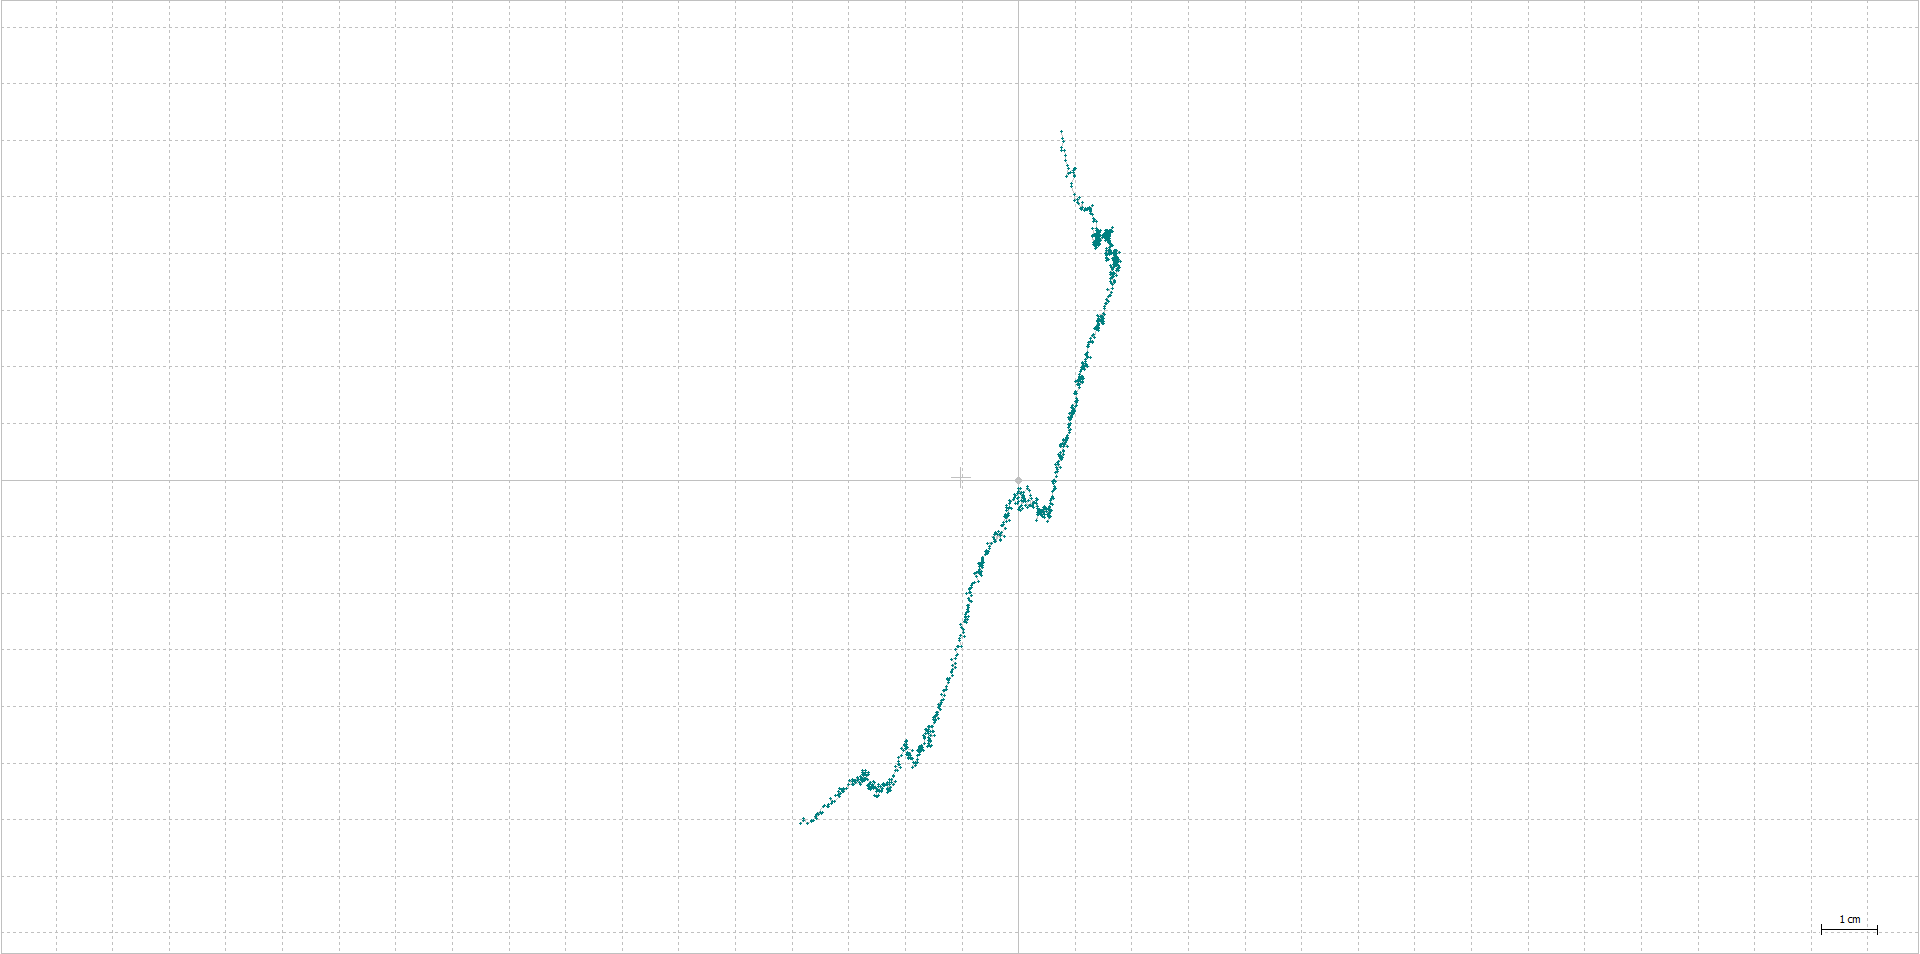
\includegraphics[width=0.45\textwidth]{A1_beidou.png}}
	\subfigure[ohne Beidou (Gitter L"anger 1mm)]{
		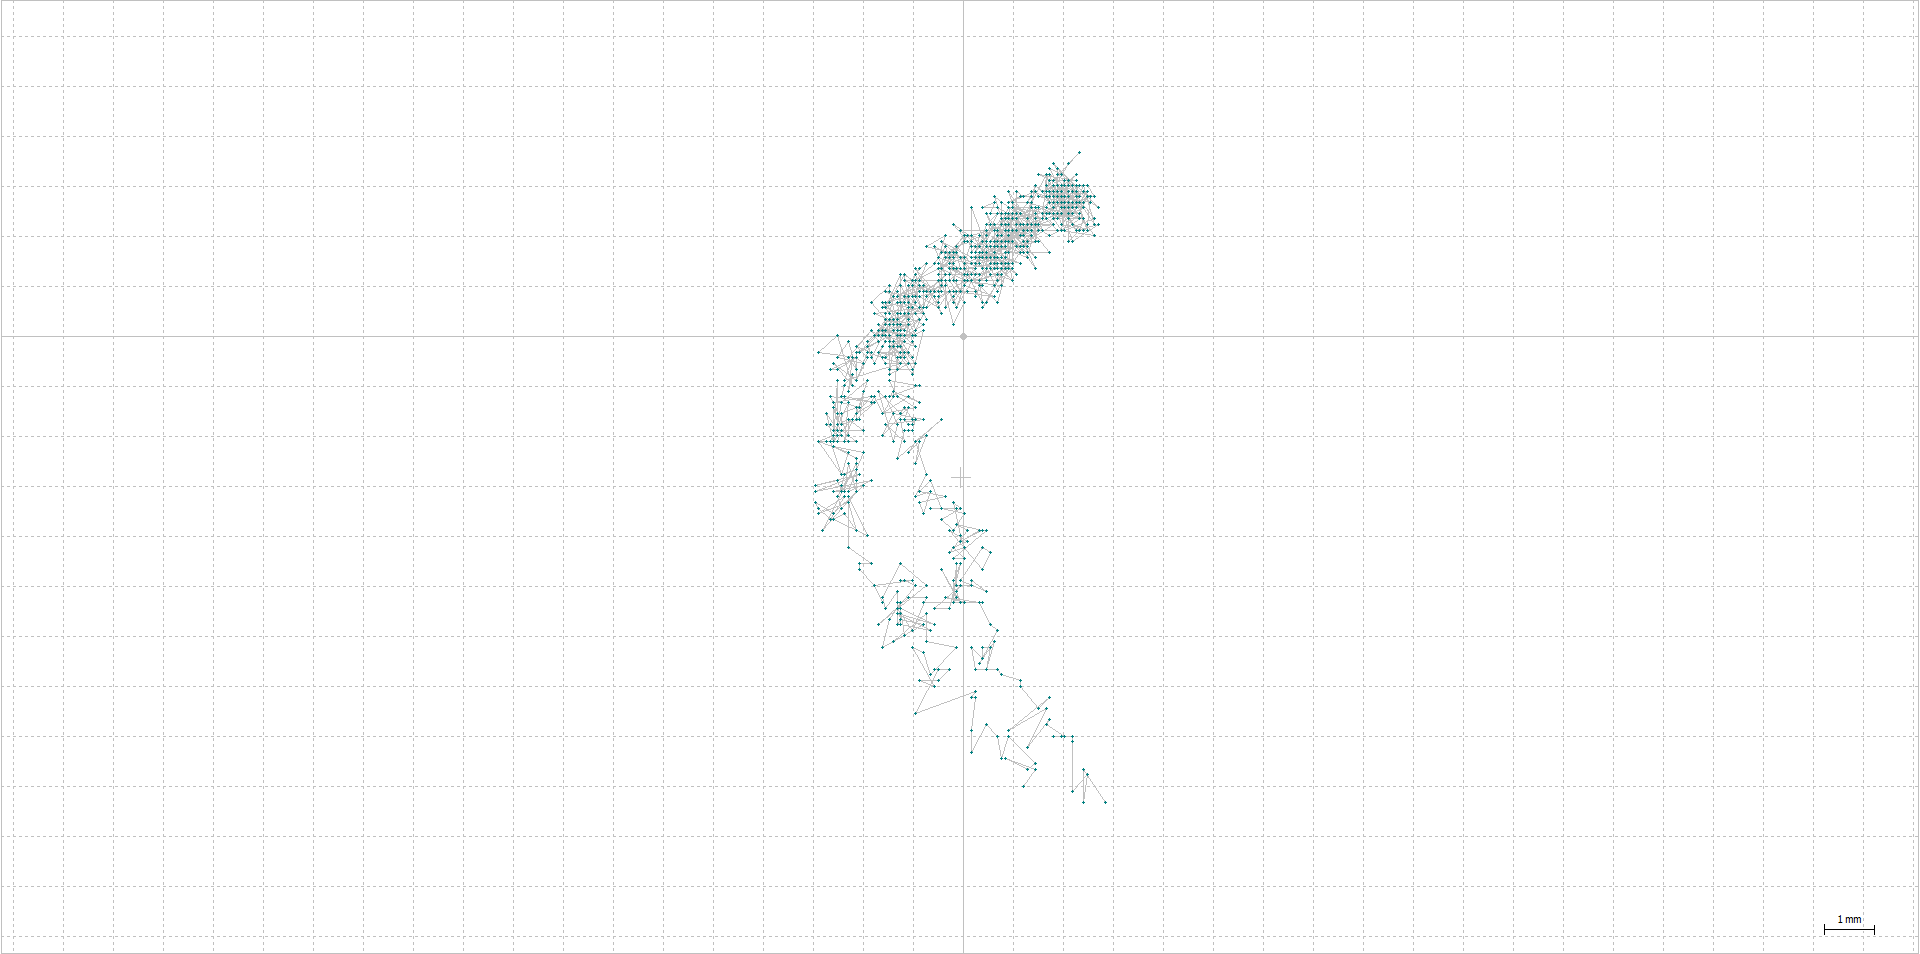
\includegraphics[width=0.45\textwidth]{A1_lauf.png}}
	\caption{Gound Track}
	\label{fig:bewegung}
\end{figure}\\
Die Position ist relativ konstant, Die Koordinaten liegt in \autoref{fig:pos}, es ist zu sehen, dass die Abweichung in Vertikale Richtung deutlich h"oher als in Horizontal Richtungen. 
\begin{figure}[ht]\centering 
	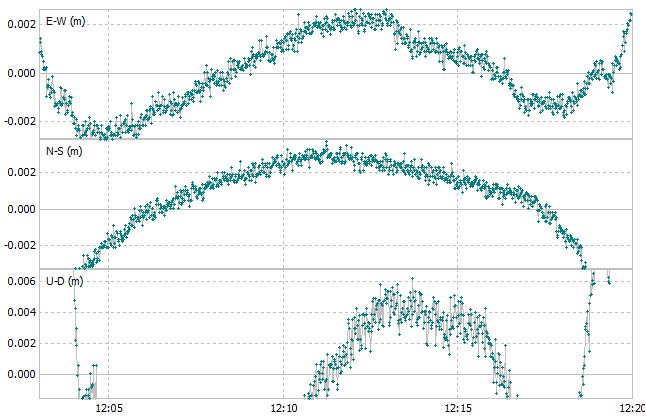
\includegraphics[width=0.9\textwidth]{A1_Pos.png}
	\caption{Position}
	\label{fig:pos}
\end{figure}\\\\
In \autoref{fig:velacc} liegt die Geschwindigkeit und Beschleunigung. Die werte sind gegen 0 mit zuf"alligen Abweichungen und die Abweichungen sind in H"ohen Richtung maximal. weil die Geschwindigkeit und Beschleunigung des Sensors konstant mit wei"ses Rauschen sein sollen, beeinflusst sie die Positions mit einem Integrated Random Walk.  
\begin{figure}[ht]\centering 
	\subfigure[Geschwindigkeit]{
		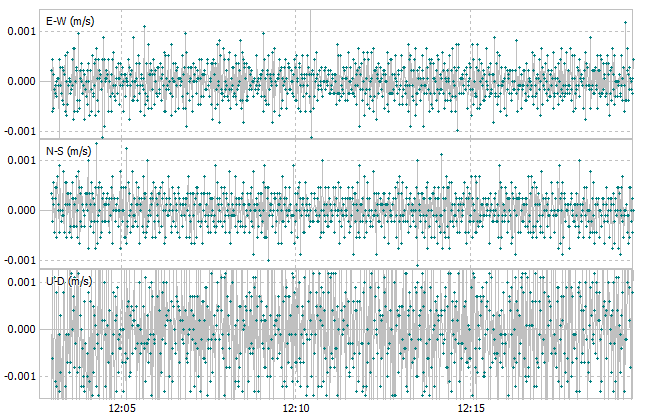
\includegraphics[width=0.9\textwidth]{A1_Vel.png}}
	\subfigure[Beschleunigung]{
		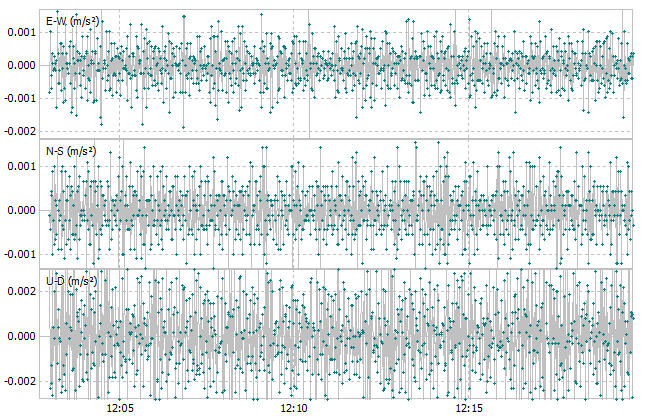
\includegraphics[width=0.9\textwidth]{A1_Acc.png}}
	\caption{}
	\label{fig:velacc}
\end{figure}\\\\
Wenn man nach die Standardabweichungen der Position schaut, ist es zu sehen, dass je weit die Position von 0 abreichert, desto gr"o"ser ist die Standardabweichung.\autoref{fig:std}
\begin{figure}[ht]\centering 
	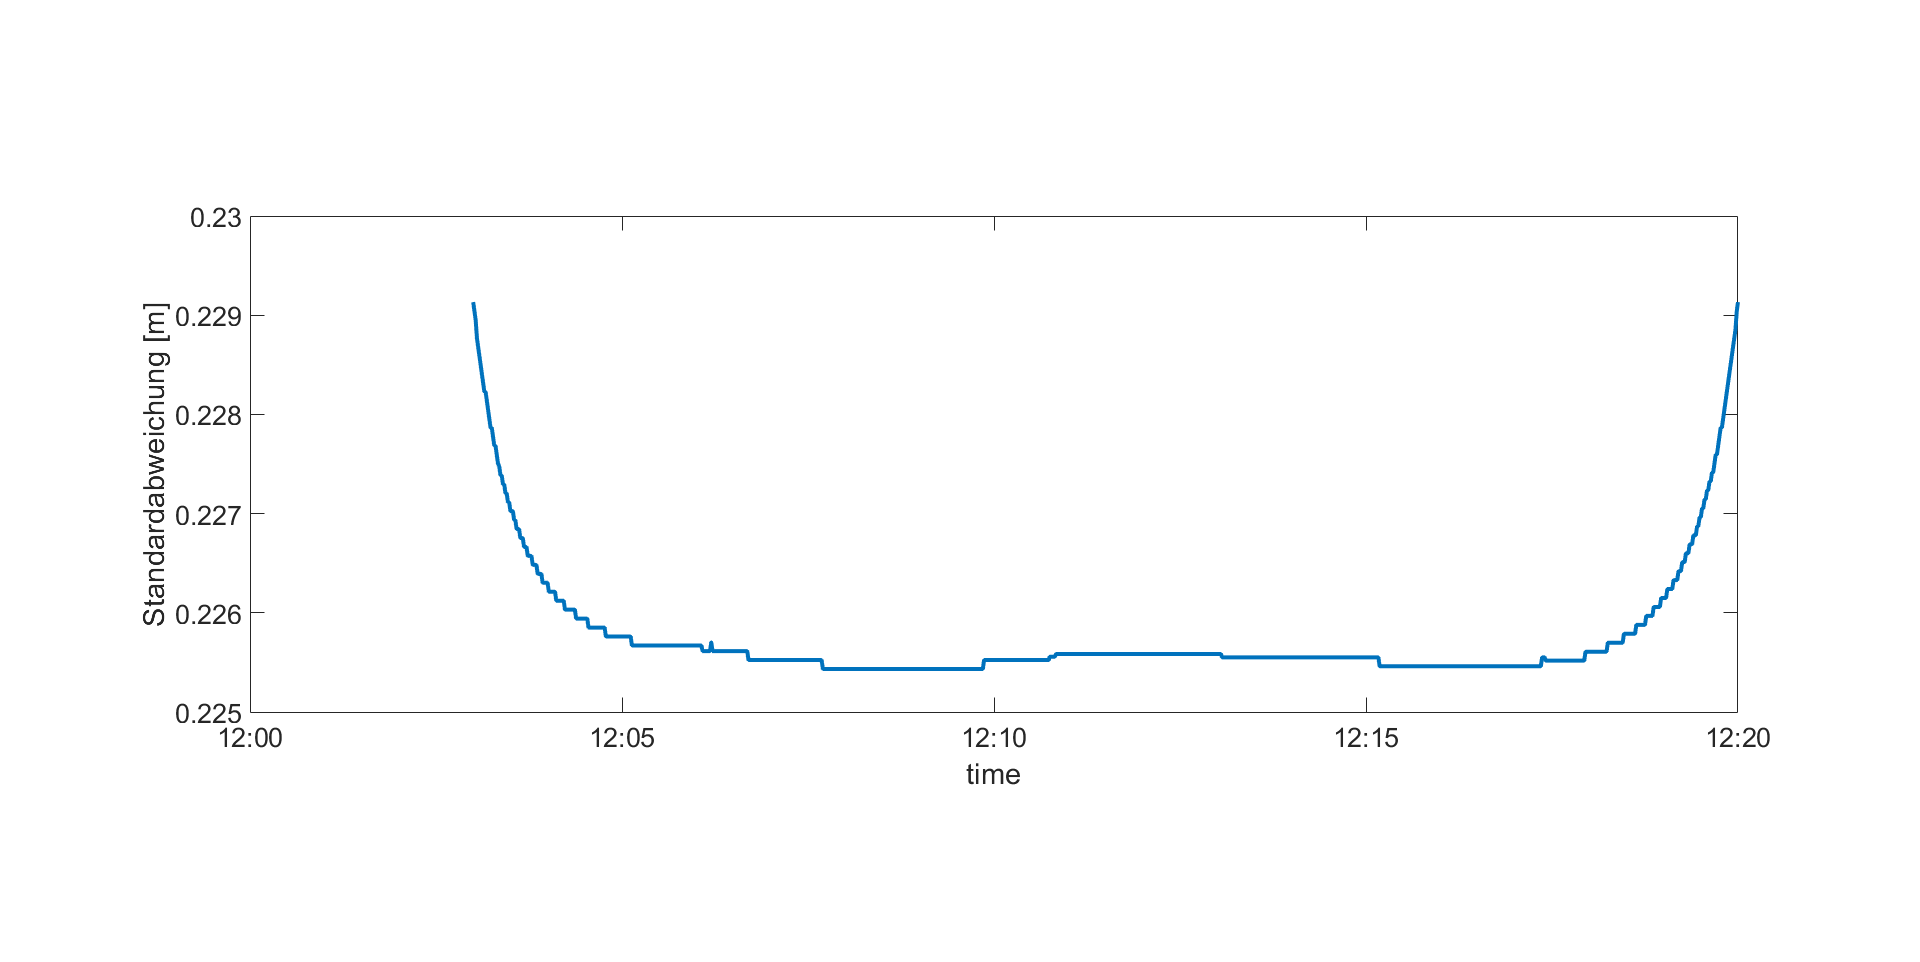
\includegraphics[width=0.9\textwidth]{A1_std.png}
	\caption{Standardabweichung Position}
	\label{fig:std}
\end{figure}\\\\
Die Residuen \autoref{fig:residuen} von Tr"agerphasen sind in manchen Elevationsbereich besonders gro"s, weil das Signal in diesen Bereichen nicht direkt am Empf"anger gelangt. 
\begin{figure}[ht]\centering 
	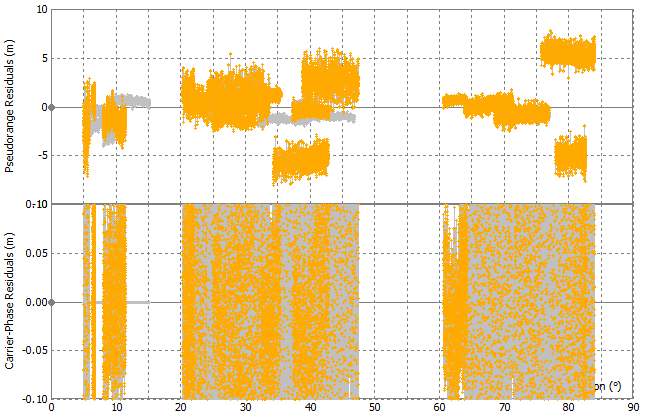
\includegraphics[width=0.9\textwidth]{A1_res.png}
	\caption{Residuen}
	\label{fig:residuen}
\end{figure}
\clearpage


\section{Aufgabe 2}
In dieser Teile sind die Position von Flugzeug mit PPP kinematisch Verfahren bestimmt werden. Die Trajektorie sieht "ahnlich wie bei "Ubung 2 aus. \autoref{fig:A2lauf}. Die Form der Standardabweichung ist auch "ahnlich, aber die Werte sind mehrfach gr"o"ser in Meterbereich. \autoref{fig:std2}
\begin{figure}[ht]\centering 
	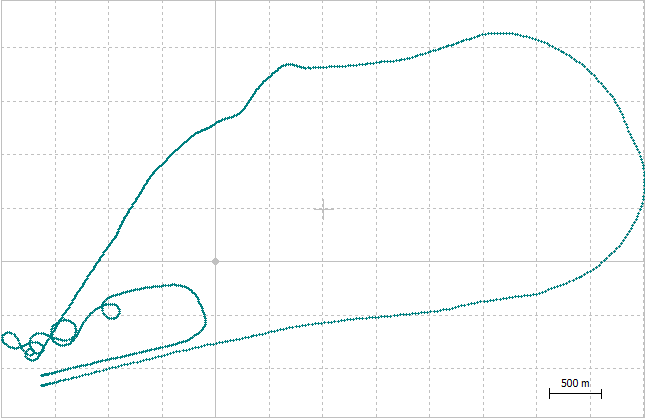
\includegraphics[width=0.7\textwidth]{A2_lauf.png}
	\caption{Trajektorie}
	\label{fig:A2lauf}
\end{figure}
\begin{figure}[ht]\centering 
	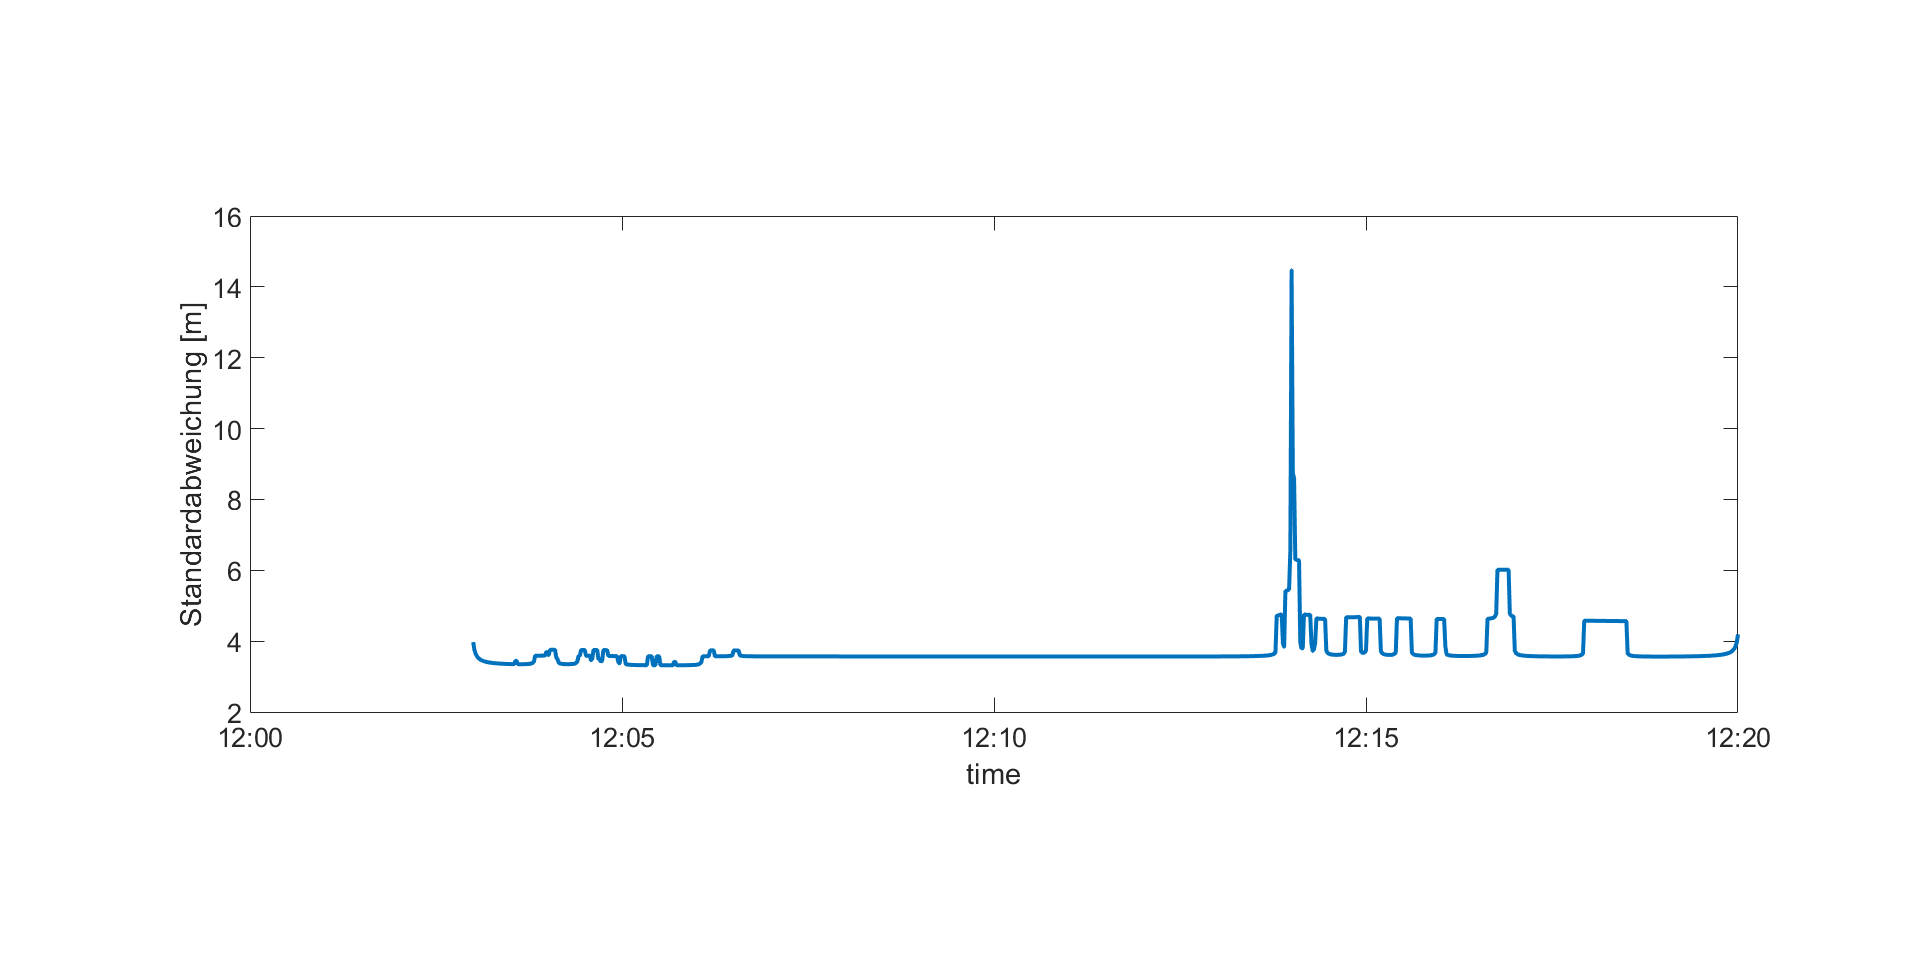
\includegraphics[width=0.9\textwidth]{A2_std.png}
	\caption{Standardabweichung}
	\label{fig:std2}
\end{figure}
\clearpage


\section{Aufgabe 3}
In dieser Teile ist die Ergebnisse von RTKlib mit der von CSRS-PPP verglichen. Der Vergleich von PPP statisch liegt in \autoref{fig:A3_stat} und von kinematisch in \autoref{fig:A3_kine} und \autoref{fig:A3_kine2}.
\begin{figure}[ht]\centering 
	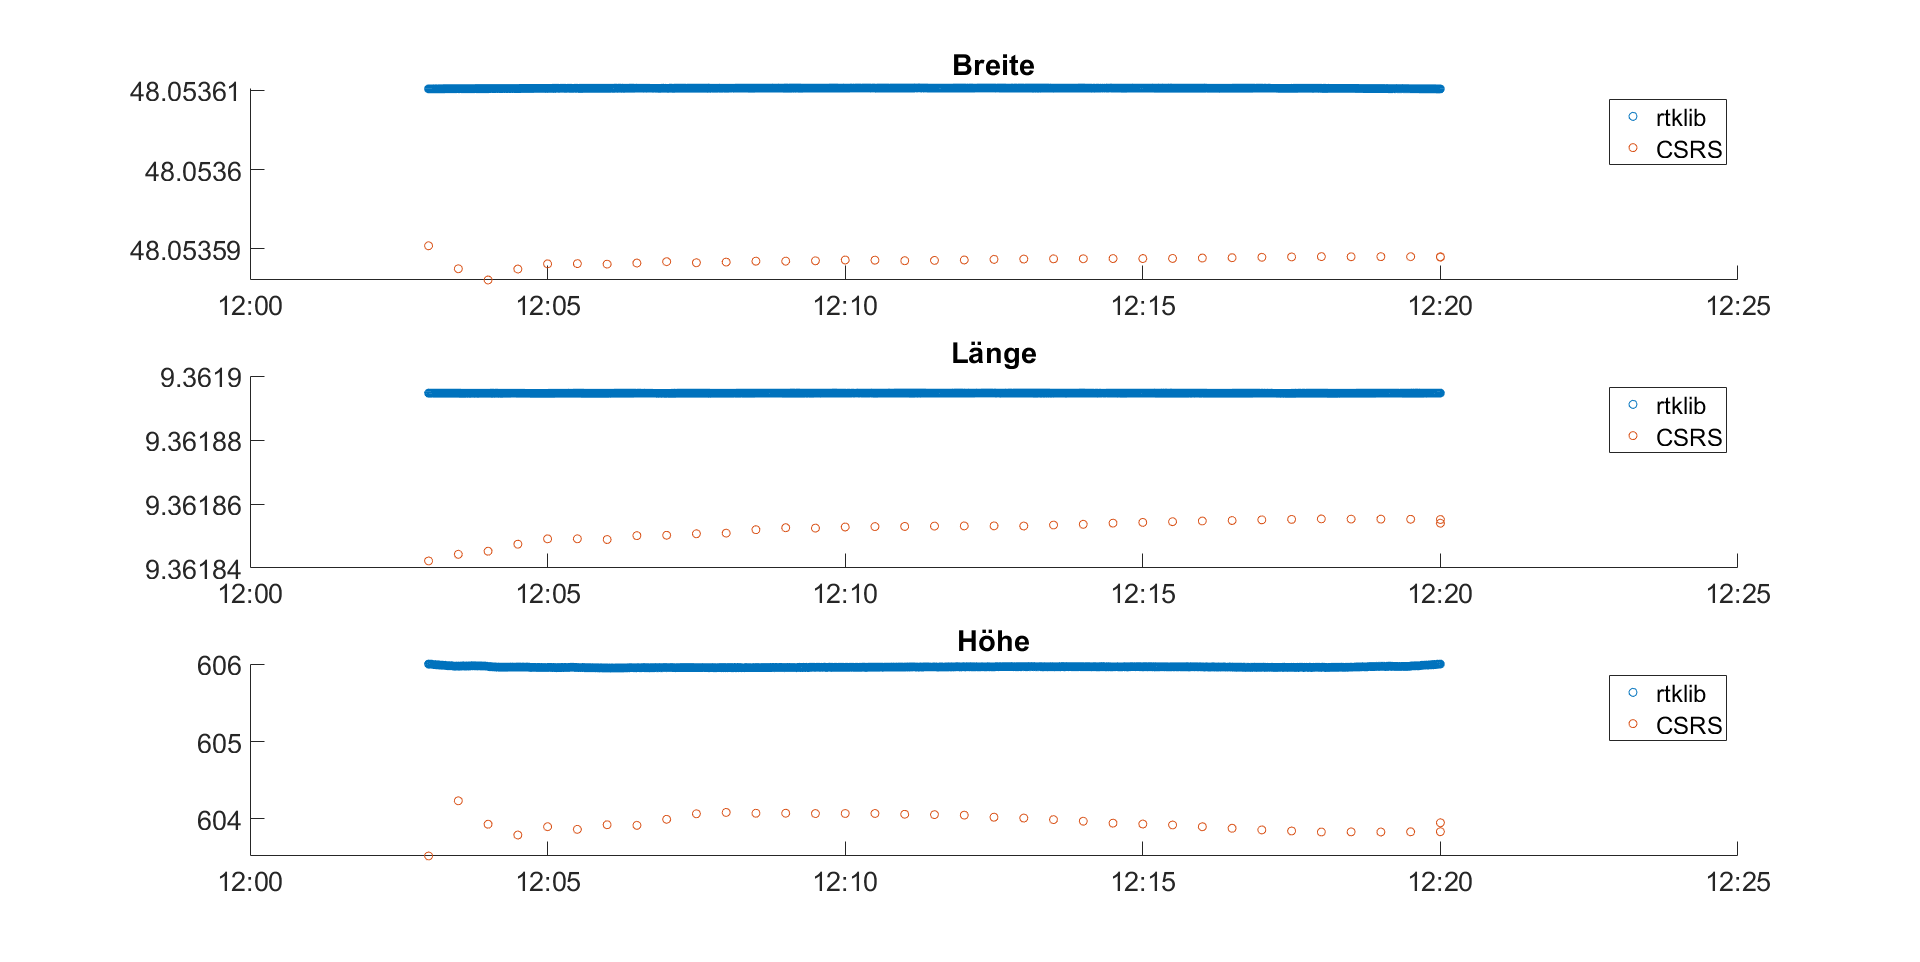
\includegraphics[width=0.9\textwidth]{A3_statisch.png}
	\caption{Statisch PPP}
	\label{fig:A3_stat}
\end{figure}
\begin{figure}[ht]\centering 
	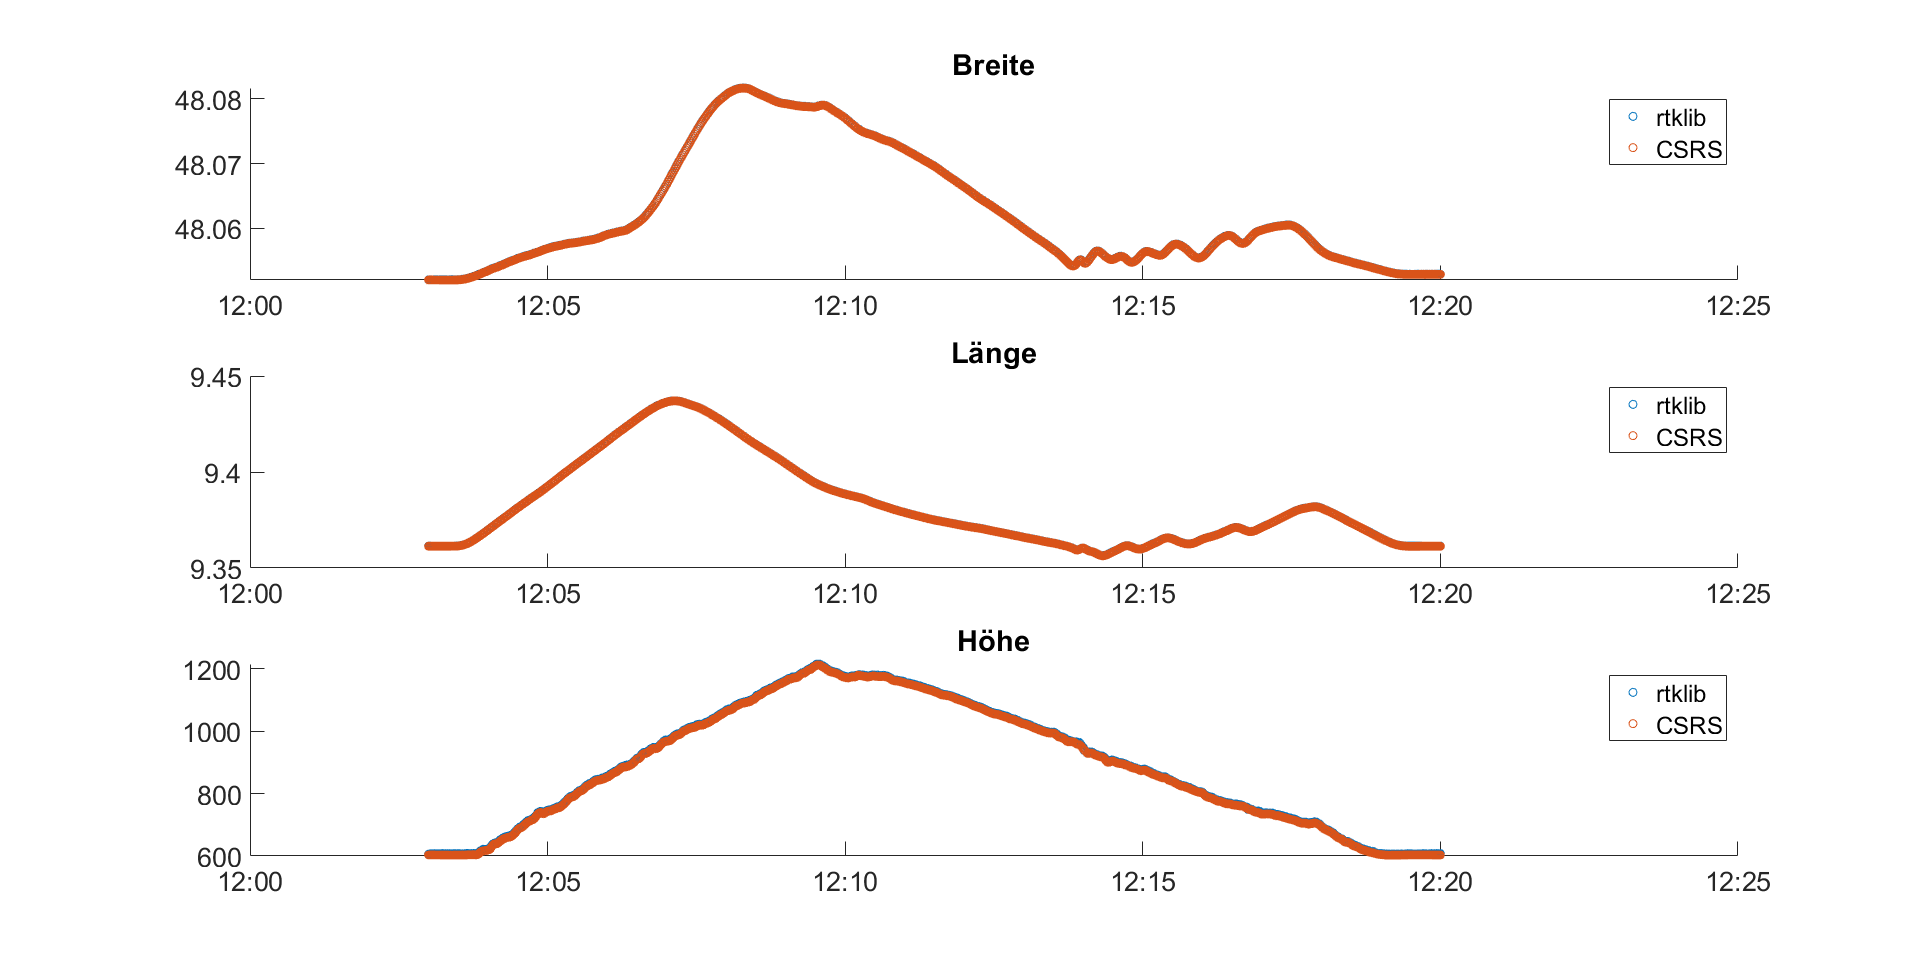
\includegraphics[width=0.9\textwidth]{A3_kinematisch.png}
	\caption{Kinematisch PPP}
	\label{fig:A3_kine}
\end{figure}\\\\
Bei beiden Verfahren sind die Differenz am Horizontal Richtungen sehr klein in Grad, aber wenn man diesen Unterschied nach Meter umrechnen, ist die Unterschied von beiden Verfahren in Meterbereich wie in vertikale Richtung.\autoref{fig:A3_kine2}. Die Ergebnisse von beiden Softwares haben eine deutliche Werteunterschied obwhol die Tendenz "ahnlich ist. 
\begin{figure}[ht]\centering 
	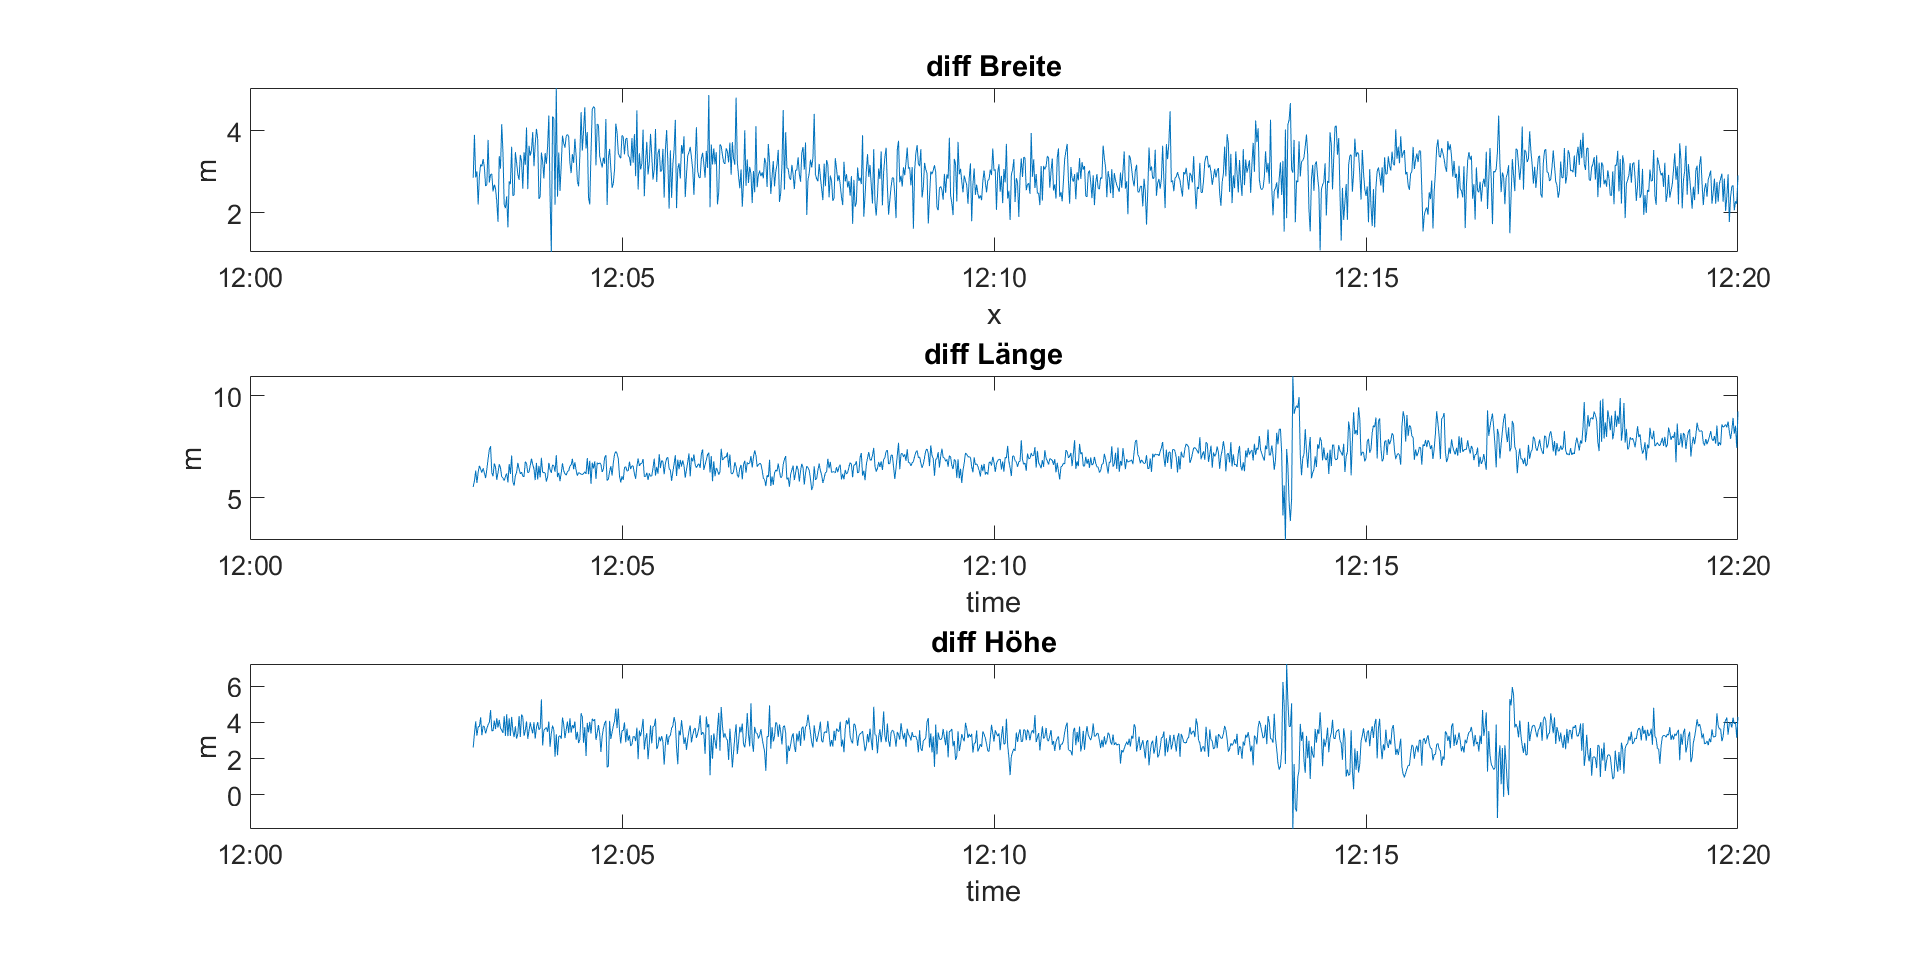
\includegraphics[width=0.9\textwidth]{A3_kine2.png}
	\caption{Differenz Kinematisch PPP}
	\label{fig:A3_kine2}
\end{figure}